\documentclass[a4paper,graphics,11pt]{article}
\pagenumbering{arabic}

\usepackage[margin=1in]{geometry}
\usepackage[utf8]{inputenc}
\usepackage[T1]{fontenc}
\usepackage{lmodern}
\usepackage[ngerman]{babel}
\usepackage{amsmath, tabu}
\usepackage{amsthm}
\usepackage{amssymb}
\usepackage{complexity}
\usepackage{mathtools}
\usepackage{setspace}
\usepackage{graphicx,color,curves,epsf,float,rotating}
\usepackage{tasks}
\setlength{\parindent}{0em}
\setlength{\parskip}{1em}

\newcommand{\aufgabe}[1]{\subsection*{Aufgabe #1}}
\newcommand{\up}[2]{\mathrel{\overset{\makebox[0pt]{\mbox{\normalfont\tiny #2}}}{#1}}}
\newcommand{\re}{\operatorname{Re}}
\newcommand{\im}{\operatorname{Im}}

\begin{document}
\noindent Gruppe \fbox{\textbf{11}}             \hfill Tobias Riedel, 379133 \\
\noindent Analysis für Informatiker             \hfill Phil Pützstück, 377247 \\
\begin{center}
	\LARGE{\textbf{Hausaufgabe 8}}
\end{center}
\begin{center}
\rule[0.1ex]{\textwidth}{1pt}
\end{center}



\aufgabe{1}
\textbf{a)}\\[5pt]
Für $w_1$ gilt:
$$
    w_1 = \frac{2}{1-3i}
    = (2+0i)\cdot (1-3i)^{-1}
    = (2+0i) \cdot \left(\frac{1+3i}{1^2+3^2}\right)
    = (2+0i) \cdot \left(\frac{1}{10} + \frac{3}{10}i\right)
    = \frac{1}{5} + \frac{3}{5}i
$$
Es folgt
$$
    \re(w_1) = \frac{1}{5} \quad \text{und}\quad \im(w_1) = \frac{3}{5}
$$

Für $w_2$ gilt:
$$
    w_2 = \frac{1}{i}
    = (1+0i)\cdot (0+i)^{-1}
    = (1+0i)\cdot\left(\frac{0-i}{1}\right)
    = 0-i
$$
Es folgt
$$
    \re(w_2) = 0 \quad \text{und}\quad \im(w_2) = -1
$$

Für $w_3$ gilt:
$$
    w_3 = \frac{1+it}{1-it}
$$
Es folgt
$$
    \re(w_3) = \quad \text{und}\quad \im(w_3) = 
$$

\textbf{b)}
Nach Satz \textbf{???} lässt sich der Betrag $|z|$ wie folgt berechnen:
$$
    \left|\frac{(3+4i)(-1+2i)}{(-1-i)(3-i)}\right|
    = \frac{|(3+4i)(-1+2i)|}{|(-1-i)(3-i)|}
    =\frac{|3+4i|\cdot|-1+2i|}{|-1-i|\cdot|3-i|} 
    = \frac{5\cdot\sqrt{5}}{\sqrt{2}\cdot\sqrt{10}} = \frac{5}{2}
$$

\textbf{c)}
Sei $x,y \in \mathbb{R}$ mit $z=x+iy$. Es gilt
$$
    \left|\frac{z+i}{z-i}\right|
    = \frac{|z+i|}{|z-i|}
    = \frac{|(x+iy)+i|}{|(x+iy)-i|}
    = \frac{|x+i(y+1)|}{|x+i(y-1)|}
    = \sqrt{\frac{x^2+(y+1)^2}{x^2+(y-1)^2}}
    \leq 1
$$
Die lässt sich weiter umformen:
$$
    \sqrt{\frac{x^2+(y+1)^2 }{x^2+(y-1)^2}} \leq 1
    \,\Longleftrightarrow\, \frac{x^2+(y+1)^2}{x^2+(y-1)^2} \leq 1^2 = 1
    \,\Longleftrightarrow\, x^2+(y+1)^2 \leq x^2+(y-1)^2
$$$$
    \,\Longleftrightarrow\, (y^2+2y+1)-(y^2-2y+1) \leq 0
    \,\Longleftrightarrow\, 4y \leq 0
    \,\Longleftrightarrow\, y \leq 0
$$
Also ist die Ungleichung für alle $z \in \mathbb{C}$ mit $\im(z) \leq 0$ erfüllt.

\newpage

\textbf{d)}
Sei $x,y \in \mathbb{R}$ mit $z=x+iy$. Es gilt
$$
    \frac{1+z}{1-z}
    = \frac{1+(x+iy)}{1-(x+iy)}
    = 
$$

\aufgabe{2}
Sei $x,y \in \mathbb{R}$ mit $z = x+iy$.

\textbf{a)}
Durch $|z| = \sqrt{x^2+y^2}$ folgt
\begin{center}
    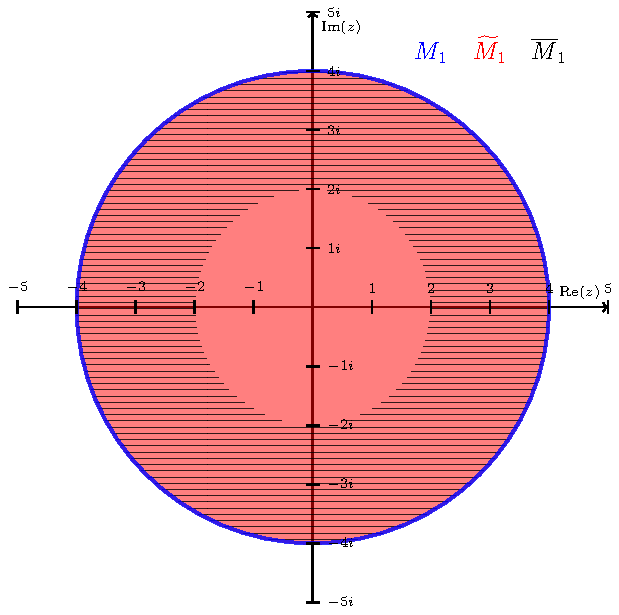
\includegraphics{graphics/graph1.pdf}
\end{center}

\textbf{b)}
$$
    2\re(z) + 5\im(y) = 1
    \,\Longleftrightarrow\, 2x+5y = 1
    \,\Longleftrightarrow\, y = \frac{1-2x}{5}
$$

\textbf{c)}
$$
    \re(z) + \im(z) -1 > 2
    \,\Longleftrightarrow\, x+y > 3
    \,\Longleftrightarrow\, y > 3-x
$$

\textbf{d)}
$$
    (\re(z) \geq 0) \land (|z|\leq 9) \land (\re(z) \leq \im(z)
    \,\Longleftrightarrow\, (0 \leq x \leq y) \land \left(\sqrt{x^2+y^2} < 9\right)
$$






\end{document}
